\documentclass[../thesis.tex]{subfiles}

\begin{document}

\appendix

\chapter{Data Description}
\label{chap:data_desc}

\noindent In this appendix we present a descriptive overview of the data used in this thesis. This includes: an overview and explanation of the variables used (\ref{sec:variables}), the \texttt{R}-packages (\ref{sec:r_pack}) used and some relevant plots (\ref{sec:rel_plots}) to support the finding in the thesis. The source code used to produce the relevant plots can be found in appendix (\ref{chap:souce_code}).  

\section{Variables}
\label{sec:variables}

\section{\texttt{R}-packages}
\label{sec:r_pack}

\section{Descriptive Statistics}
\label{sec:desc_stat}


\begin{scriptsize}
\begin{tabularx}{\textwidth}{P{3cm}rrrrrrrrrr}
\caption{Patient characteristics: HFpEF}\label{tab:desc_stat_HFpEF_variables}\\
\toprule
\textbf{Variable} & $n$ & \#Na & Min & Max & $\bar{x}$ & $\widetilde{x}$ & $s$ & $q_1$ & $q_3$ \\ 
\midrule
\endfirsthead
\caption*{\textbf{Table \ref{tab:desc_stat_HFpEF_variables}:} Patient characteristics: HFpEF (\textit{continued})}\\
\toprule
 \textbf{Variable} & $n$ & \#Na & Min & Max & $\bar{x}$ & $\widetilde{x}$ & $s$ & $q_1$ & $q_3$ \\ 
\midrule
\endhead
\multicolumn{10}{c}{PANEL II: Demographics}\\
\midrule
  age & 193 &   0 &  29.0 &   100.8 &   76.3 &   78.9 &   12.1 &  69.5 &   85.4 \\ 
  gender & 193 &   0 &   0.0 &     1.0 &    0.6 &    1.0 &    0.5 &   0.0 &    1.0 \\ 
  white & 193 &   0 &   0.0 &     1.0 &    0.7 &    1.0 &    0.5 &   0.0 &    1.0 \\ 
  asian & 193 &   0 &   0.0 &     1.0 &    0.1 &    0.0 &    0.2 &   0.0 &    0.0 \\ 
  black & 193 &   0 &   0.0 &     1.0 &    0.3 &    0.0 &    0.4 &   0.0 &    1.0 \\
\midrule
\multicolumn{10}{c}{PANEL III: Admission symptoms}\\
\midrule
  breathless & 185 &   8 &   0.0 &     1.0 &    0.8 &    1.0 &    0.4 &   1.0 &    1.0 \\ 
\midrule
\multicolumn{10}{c}{PANEL IV: Admission signs}\\
\midrule
  sbp & 182 &  11 &  55.0 &   242.0 &  146.9 &  145.0 &   31.7 & 125.0 &  167.0 \\ 
  dbp & 183 &  10 &  25.0 &   195.0 &   80.5 &   80.0 &   22.1 &  67.0 &   89.0 \\ 
  admissionwgt & 160 &  33 &  41.5 &   158.0 &   78.9 &   76.7 &   23.3 &  60.1 &   93.9 \\ 
  bp & 192 &   1 &   0.0 &     1.0 &    0.8 &    1.0 &    0.4 &   1.0 &    1.0 \\ 
  bmiadmission & 148 &  45 &  16.8 &   107.1 &   30.7 &   29.3 &   10.5 &  23.6 &   35.4 \\ 
  pulse & 182 &  11 &  44.0 &   211.0 &   84.7 &   83.0 &   22.1 &  70.0 &   95.0 \\
\midrule
\multicolumn{10}{c}{PANEL V: Risk factors}\\
\midrule
  a-fib & 189 &   4 &   0.0 &     1.0 &    0.5 &    0.0 &    0.5 &   0.0 &    1.0 \\ 
  copdasthma & 190 &   3 &   0.0 &     1.0 &    0.4 &    0.0 &    0.5 &   0.0 &    1.0 \\ 
  irondef &  69 & 124 &   0.0 &     1.0 &    0.6 &    1.0 &    0.5 &   0.0 &    1.0 \\ 
  dm & 188 &   5 &   0.0 &     1.0 &    0.5 &    1.0 &    0.5 &   0.0 &    1.0 \\ 
  obesity & 185 &   8 &   0.0 &     1.0 &    0.5 &    1.0 &    0.5 &   0.0 &    1.0 \\ 
  copdasthma.1 & 190 &   3 &   0.0 &     1.0 &    0.4 &    0.0 &    0.5 &   0.0 &    1.0 \\ 
  ihd & 186 &   7 &   0.0 &     1.0 &    0.4 &    0.0 &    0.5 &   0.0 &    1.0 \\ 
\midrule
\multicolumn{10}{c}{PANEL VI: Comorbidities}\\
\midrule
  comorbidities & 193 &   0 &   0.0 &     9.0 &    4.2 &    4.0 &    1.8 &   3.0 &    5.0 \\ 
\midrule
\multicolumn{10}{c}{PANEL VII: Electrocardiography}\\
\midrule
  ecgqrsduration & 157 &  36 &  55.0 &   177.0 &  101.3 &   98.0 &   20.8 &  88.0 &  112.0 \\ 
  ecgqrsother & 193 &   0 &   0.0 &     1.0 &    0.0 &    0.0 &    0.2 &   0.0 &    0.0 \\ 
  ecgrate & 159 &  34 &  41.0 &   191.0 &   83.0 &   80.0 &   23.1 &  70.0 &   92.0 \\ 
  ecgrhythmother & 193 &   0 &   0.0 &     1.0 &    0.1 &    0.0 &    0.2 &   0.0 &    0.0 \\ 
  lvh & 169 &  24 &   0.0 &     1.0 &    0.1 &    0.0 &    0.3 &   0.0 &    0.0 \\ 
  normalecgqrs & 193 &   0 &   0.0 &     1.0 &    0.6 &    1.0 &    0.5 &   0.0 &    1.0 \\ 
  lbbb & 193 &   0 &   0.0 &     1.0 &    0.0 &    0.0 &    0.2 &   0.0 &    0.0 \\ 
  rbbb & 193 &   0 &   0.0 &     1.0 &    0.1 &    0.0 &    0.3 &   0.0 &    0.0 \\ 
  sr & 193 &   0 &   0.0 &     1.0 &    0.6 &    1.0 &    0.5 &   0.0 &    1.0 \\
\midrule
\multicolumn{10}{c}{PANEL VIII: Laboratory tests}\\
\midrule
  hb & 192 &   1 &  47.0 &   185.0 &  107.6 &  107.5 &   21.1 &  91.8 &  123.0 \\ 
  wbc & 192 &   1 &   2.9 &   209.4 &   10.2 &    7.6 &   15.8 &   6.0 &   10.5 \\ 
  tsat &  94 &  99 &   4.0 &    92.0 &   20.4 &   18.0 &   13.8 &  11.0 &   24.8 \\ 
  plts & 192 &   1 &  51.0 &   497.0 &  229.4 &  217.0 &   89.5 & 163.0 &  284.2 \\ 
  pcv & 193 &   0 &   0.2 &     0.6 &    0.3 &    0.3 &    0.1 &   0.3 &    0.4 \\ 
  ferritin &  71 & 122 &   9.0 &  2223.0 &  378.2 &  173.0 &  533.8 &  61.5 &  443.5 \\ 
  k & 189 &   4 &   2.4 &     8.7 &    4.4 &    4.4 &    0.6 &   4.1 &    4.7 \\ 
  ironlevels &  95 &  98 &   2.0 &    23.0 &    8.6 &    7.0 &    4.8 &   5.0 &   11.0 \\ 
  chol & 190 &   3 &   0.0 &     1.0 &    0.5 &    1.0 &    0.5 &   0.0 &    1.0 \\ 
  ntprobnp & 193 &   0 &  81.0 & 70000.0 & 5047.3 & 2217.0 & 8487.4 & 997.0 & 5305.0 \\ 
  gfr & 193 &   0 &   3.0 &   221.0 &   54.1 &   47.0 &   31.1 &  32.0 &   72.0 \\ 
  mcv & 193 &   0 &  57.0 &   117.0 &   88.8 &   89.0 &    8.9 &  85.0 &   94.0 \\ 
  na & 193 &   0 & 110.0 &   148.0 &  138.2 &  139.0 &    4.9 & 136.0 &  141.0 \\
\midrule
\multicolumn{10}{c}{PANEL IX: Echocardiography}\\
\midrule
  lvef & 191 &   2 &  50.0 &    72.5 &   57.1 &   57.5 &    4.5 &  55.0 &   60.0 \\ 
  ewave & 174 &  19 &   0.4 &     1.6 &    0.9 &    0.9 &    0.3 &   0.7 &    1.1 \\ 
  pasp & 122 &  71 &  14.0 &    85.0 &   43.5 &   42.5 &   14.2 &  34.0 &   51.8 \\ 
  ee & 152 &  41 &   2.0 &    37.0 &   13.4 &   12.5 &    5.8 &   9.0 &   16.0 \\ 
  mr & 193 &   0 &   0.0 &     2.0 &    0.5 &    0.0 &    0.7 &   0.0 &    1.0 \\ 
  tr & 193 &   0 &   0.0 &     3.0 &    0.9 &    1.0 &    0.8 &   0.0 &    1.0 \\ 
  as & 193 &   0 &   0.0 &     2.0 &    0.1 &    0.0 &    0.3 &   0.0 &    0.0 \\ 
  ai & 193 &   0 &   0.0 &     2.0 &    0.2 &    0.0 &    0.5 &   0.0 &    0.0 \\ 
  rvfunction & 192 &   1 &   0.0 &     4.0 &    0.6 &    0.0 &    1.2 &   0.0 &    0.2 \\ 
  af & 193 &   0 &   0.0 &     1.0 &    0.2 &    0.0 &    0.4 &   0.0 &    0.0 \\ 
\midrule
\multicolumn{10}{c}{PANEL X: Outcomes}\\
\midrule
  timetohfadm &  69 & 124 &   3.8 &   718.8 &  192.5 &  122.7 &  197.8 &  33.0 &  270.0 \\ 
  hfhospitalisation & 193 &   0 &   0.0 &     1.0 &    0.4 &    0.0 &    0.5 &   0.0 &    1.0 \\ 
  los & 171 &  22 &   1.0 &   372.0 &   15.8 &    8.0 &   31.3 &   4.0 &   19.0 \\ 
\midrule
\end{tabularx}
\end{scriptsize}


\begin{scriptsize}
\begin{tabularx}{\textwidth}{P{3cm}RRRRRRRRRR}
\caption{Patient characteristics: HFmrEF}\label{tab:desc_stat_HFmrEF_variables}\\
\toprule
\textbf{Variable}\parnote{\scriptsize Note: $n$ - number of observations, \#Na - number of missing data, Min - minimal, Max - maximal,  $\bar{x}$ - arithmetic mean, $\widetilde{x}$ - median, $s$ - standard deviation, $q_1$ - first quartile and $q_3$ - third quartile.} & $n$ & \# Na & Min & Max & $\bar{x}$ & $\widetilde{x}$ & $s$ & $q_1$ & $q_3$ \\ 
\midrule
\endfirsthead
\caption*{\textbf{Table \ref{tab:desc_stat_HFmrEF_variables}:} Patient characteristics: HFmrEF (\textit{continued})}\\
\toprule
 \textbf{Variable} & $n$ & \#Na & Min & Max & $\bar{x}$ & $\widetilde{x}$ & $s$ & $q_1$ & $q_3$ \\ 
\midrule
\endhead
\multicolumn{10}{c}{PANEL I: Identification}\\
\midrule
patientid & 182 &   0 &     1.0 &    193.0 &    96.9 &    97.5 &    56.6 &    47.2 &   146.5 \\ 
\midrule
\multicolumn{10}{c}{PANEL II: Demographics}\\
\midrule
  gender & 182 &   0 &  0.0 &      1.0 &    0.4 &    0.0 &     0.5 &    0.0 &    1.0 \\ 
  white & 182 &   0 &  0.0 &      1.0 &    0.7 &    1.0 &     0.5 &    0.0 &    1.0 \\ 
  asian & 182 &   0 &  0.0 &      1.0 &    0.1 &    0.0 &     0.3 &    0.0 &    0.0 \\ 
  black & 182 &   0 &  0.0 &      1.0 &    0.2 &    0.0 &     0.4 &    0.0 &    0.0 \\
\midrule
\multicolumn{10}{c}{PANEL III: Admission symptoms}\\
\midrule
  breathless &  55 & 127 &  0.0 &      3.0 &    2.4 &    3.0 &     1.0 &    2.0 &    3.0 \\  
\midrule
\multicolumn{10}{c}{PANEL IV: Admission signs}\\
\midrule
  sbp &  98 &  84 & 86.0 &    242.0 &  132.6 &  126.5 &    27.7 &  114.2 &  147.8 \\ 
  dbp &  95 &  87 & 45.0 &    591.0 &   80.2 &   72.0 &    55.7 &   62.0 &   85.0 \\ 
  admissionwgt &  51 & 131 & 21.0 &    134.9 &   80.6 &   80.6 &    21.8 &   66.7 &   96.4 \\ 
  bp & 182 &   0 &  0.0 &      1.0 &    0.7 &    1.0 &     0.5 &    0.0 &    1.0 \\ 
  bmiadmission &   4 & 178 & 18.7 &     36.1 &   26.0 &   24.7 &     8.0 &   20.2 &   30.5 \\ 
  pulse &  98 &  84 & 54.0 &    144.0 &   88.8 &   85.0 &    21.9 &   71.2 &  100.0 \\
\midrule
\multicolumn{10}{c}{PANEL V: Risk factors}\\
\midrule
  a-fib & 182 &   0 &  0.0 &      1.0 &    0.4 &    0.0 &     0.5 &    0.0 &    1.0 \\ 
  copdasthma & 181 &   1 &  0.0 &      1.0 &    0.3 &    0.0 &     0.5 &    0.0 &    1.0 \\ 
  irondef &  52 & 130 &  0.0 &      1.0 &    0.4 &    0.0 &     0.5 &    0.0 &    1.0 \\ 
  dm & 180 &   2 &  0.0 &      1.0 &    0.4 &    0.0 &     0.5 &    0.0 &    1.0 \\ 
  obesity &  53 & 129 &  0.0 &      1.0 &    0.5 &    1.0 &     0.5 &    0.0 &    1.0 \\ 
  ihd & 181 &   1 &  0.0 &      1.0 &    0.5 &    0.0 &     0.5 &    0.0 &    1.0 \\ 
\midrule
\multicolumn{10}{c}{PANEL VI: Comorbidities}\\
\midrule
  comorbidities & 182 &   0 &  0.0 &      7.0 &    3.2 &    3.0 &     1.7 &    2.0 &    4.0 \\ 
\midrule
\multicolumn{10}{c}{PANEL VII: Electrocardiography}\\
\midrule
  ecgqrsduration &  77 & 105 & 71.0 &    182.0 &  104.9 &   99.0 &    24.0 &   88.0 &  116.0 \\ 
  ecgqrsother & 182 &   0 &  0.0 &      1.0 &    0.1 &    0.0 &     0.2 &    0.0 &    0.0 \\ 
  ecgrate &  88 &  94 & 42.0 &    135.0 &   86.2 &   83.5 &    21.5 &   72.2 &   99.2 \\ 
  ecgrhythmother & 182 &   0 &  0.0 &      1.0 &    0.0 &    0.0 &     0.1 &    0.0 &    0.0 \\ 
  lvh & 180 &   2 &  0.0 &      3.0 &    0.6 &    0.0 &     0.8 &    0.0 &    1.0 \\ 
  normalecgqrs & 182 &   0 &  0.0 &      1.0 &    0.3 &    0.0 &     0.4 &    0.0 &    1.0 \\ 
  lbbb & 182 &   0 &  0.0 &      1.0 &    0.0 &    0.0 &     0.2 &    0.0 &    0.0 \\ 
  rbbb & 182 &   0 &  0.0 &      1.0 &    0.0 &    0.0 &     0.2 &    0.0 &    0.0 \\ 
  sr & 182 &   0 &  0.0 &      1.0 &    0.0 &    0.0 &     0.2 &    0.0 &    0.0 \\
\midrule
\multicolumn{10}{c}{PANEL VIII: Laboratory tests}\\
\midrule
  hb & 168 &  14 & 54.0 &    153.0 &  110.7 &  111.0 &    19.9 &   98.0 &  125.0 \\ 
  wbc & 166 &  16 &  1.5 &     39.2 &    8.3 &    7.6 &     4.2 &    5.9 &    9.4 \\ 
  tsat &  71 & 111 &  1.0 &     65.0 &   20.4 &   19.0 &    12.5 &   14.0 &   25.0 \\ 
  plts & 166 &  16 & 55.0 &    638.0 &  203.8 &  187.0 &    92.3 &  143.2 &  246.5 \\ 
  pcv & 166 &  16 &  0.2 &      0.5 &    0.3 &    0.3 &     0.1 &    0.3 &    0.4 \\ 
  ferritin &  54 & 128 & 17.0 &   3853.0 &  370.2 &  225.0 &   556.3 &  102.8 &  448.0 \\ 
  k & 165 &  17 &  3.0 &      6.1 &    4.4 &    4.4 &     0.6 &    4.0 &    4.8 \\ 
  ironlevels &  70 & 112 &  2.0 &     41.0 &    9.5 &    8.0 &     7.1 &    5.0 &   11.0 \\ 
  chol & 181 &   1 &  0.0 &      1.0 &    0.4 &    0.0 &     0.5 &    0.0 &    1.0 \\ 
  ntprobnp & 182 &   0 &  5.0 &  70000.0 & 9604.4 & 4063.5 & 14051.2 & 1886.5 & 9968.2 \\ 
  gfr & 167 &  15 &  3.0 &    400.0 &   53.5 &   47.0 &    39.8 &   31.0 &   68.5 \\ 
  mcv & 166 &  16 & 65.0 &    112.0 &   91.0 &   92.0 &     8.4 &   86.0 &   96.0 \\ 
  na & 168 &  14 &  4.7 &    155.0 &  137.5 &  139.0 &    11.5 &  136.0 &  141.0 \\
\midrule
\multicolumn{10}{c}{PANEL IX: Echocardiography}\\
\midrule
  lvef & 182 &   0 & 40.0 &     50.0 &   44.0 &   45.0 &     2.9 &   42.0 &   47.5 \\ 
  ewave & 139 &  43 &  0.3 &      5.0 &    0.9 &    0.9 &     0.5 &    0.7 &    1.0 \\ 
  pasp &  72 & 110 & 18.0 & 251520.0 & 3856.5 &   40.0 & 29625.6 &   32.0 &   53.2 \\ 
  ee &  88 &  94 &  3.0 &     43.0 &   14.9 &   13.5 &     7.3 &    9.0 &   19.2 \\ 
  mr & 159 &  23 &  0.0 &      3.0 &    0.8 &    1.0 &     0.8 &    0.0 &    1.0 \\ 
  tr & 157 &  25 &  0.0 &      3.0 &    0.9 &    1.0 &     0.9 &    0.0 &    1.0 \\ 
  as & 140 &  42 &  0.0 &      2.0 &    0.2 &    0.0 &     0.5 &    0.0 &    0.0 \\ 
  ai & 151 &  31 &  0.0 &      3.0 &    0.3 &    0.0 &     0.5 &    0.0 &    0.0 \\ 
  rvfunction & 146 &  36 &  0.0 &      6.0 &    1.2 &    0.0 &     2.0 &    0.0 &    1.0 \\ 
  af & 182 &   0 &  0.0 &      1.0 &    0.2 &    0.0 &     0.4 &    0.0 &    0.0 \\ 
\midrule
\multicolumn{10}{c}{PANEL X: Outcomes}\\
\midrule
  timetohfadm & 122 &  60 &  0.4 &    575.9 &   84.5 &   44.9 &   109.6 &   11.9 &  114.7 \\ 
  hfhospitalisation & 182 &   0 &  0.0 &      1.0 &    0.2 &    0.0 &     0.4 &    0.0 &    0.0 \\ 
  los & 169 &  13 &  1.0 &    196.0 &   16.9 &    9.0 &    24.2 &    4.0 &   19.0 \\ 
\midrule
\end{tabularx}
\vspace*{-0,5cm}\parnotes
\end{scriptsize}

\newpage

\section{Relevant Plots}
\label{sec:rel_plots}

\begin{figure}[h!]
    \centering
    \hspace*{-1cm}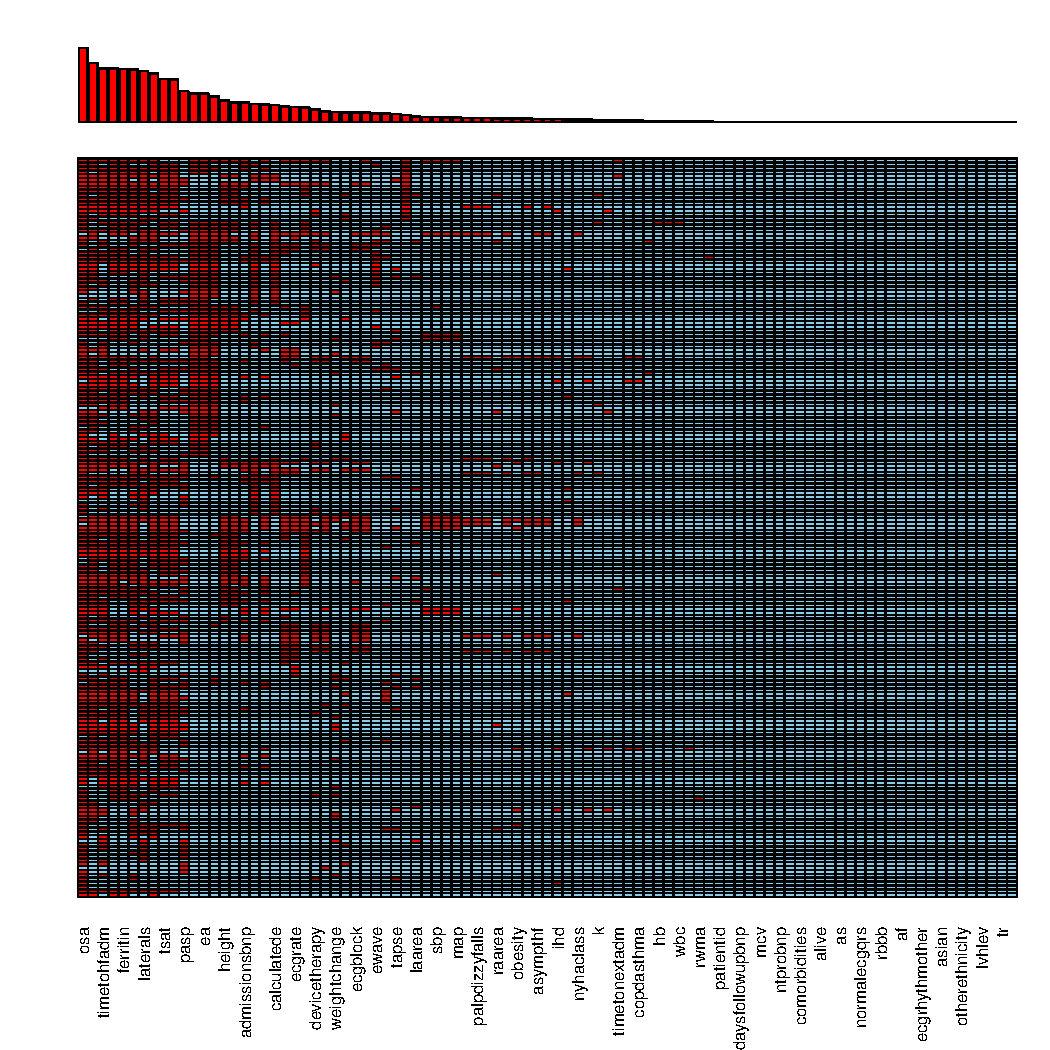
\includegraphics[width=1.1\textwidth]{doc/thesis/images/HFpEF_miss_dist.pdf}
    \caption[Missing values in HFpEF data set]{\textit{Missing values in HFpEF data set. Top:  the amount of missing values in each variable sorted in ascending order. Bottom: plot of the combinations of missing (red) and non-missing (green) values in the HFpEF data set.}}
    \label{fig:HFpEF_missing}
\end{figure}

\newpage

\begin{figure}[h!]
    \centering
    \hspace*{-1cm}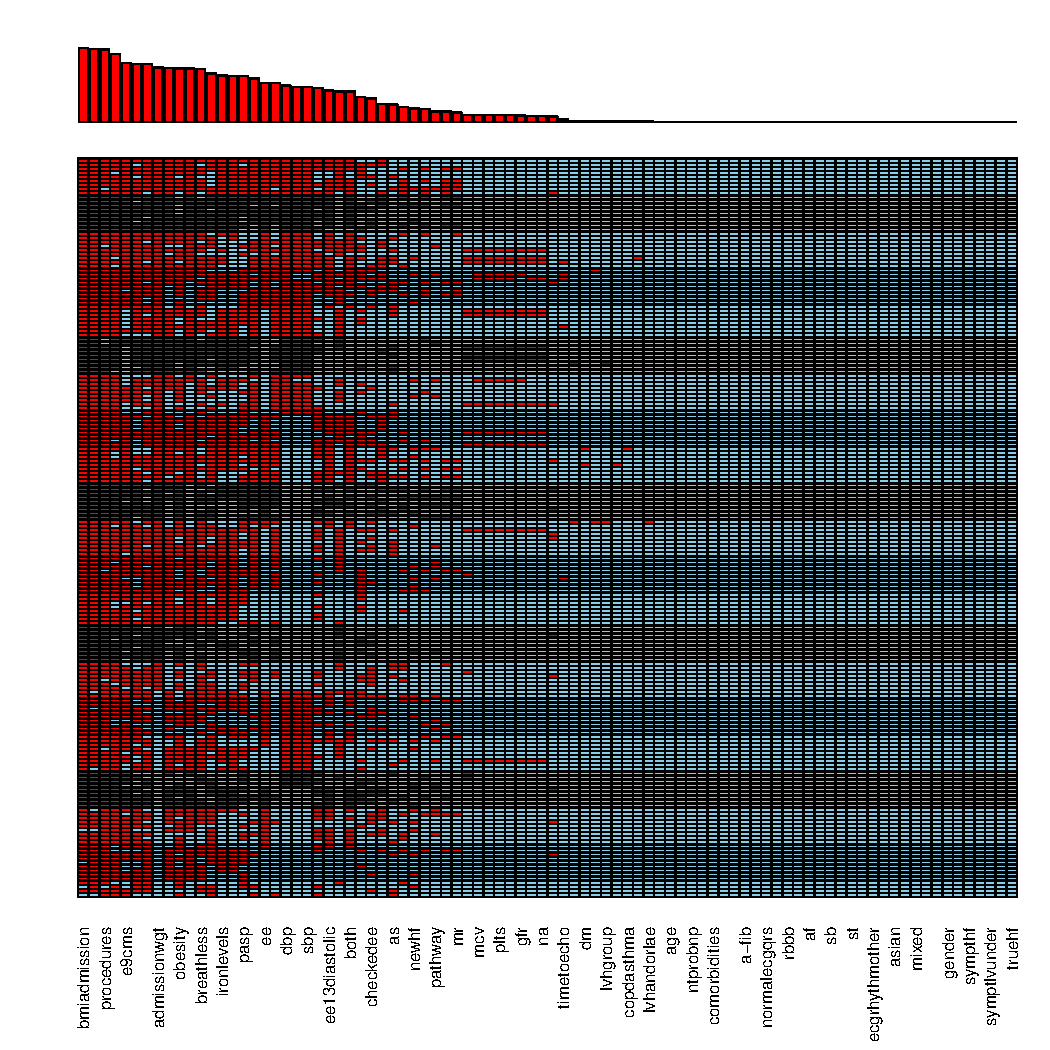
\includegraphics[width=1.1\textwidth]{doc/thesis/images/HFmrEF_miss_dist.pdf}
    \caption[Missing values in HFmrEF data set]{\textit{Missing values in HFmrEF data set. Top:  the amount of missing values in each variable sorted in ascending order. Bottom: plot of the combinations of missing (red) and non-missing (green) values in the HFmrEF data set.}}
    \label{fig:HFmrEF_missing}
\end{figure}

\newpage
\begin{figure}[h!]
    \centering
    \hspace*{-1cm}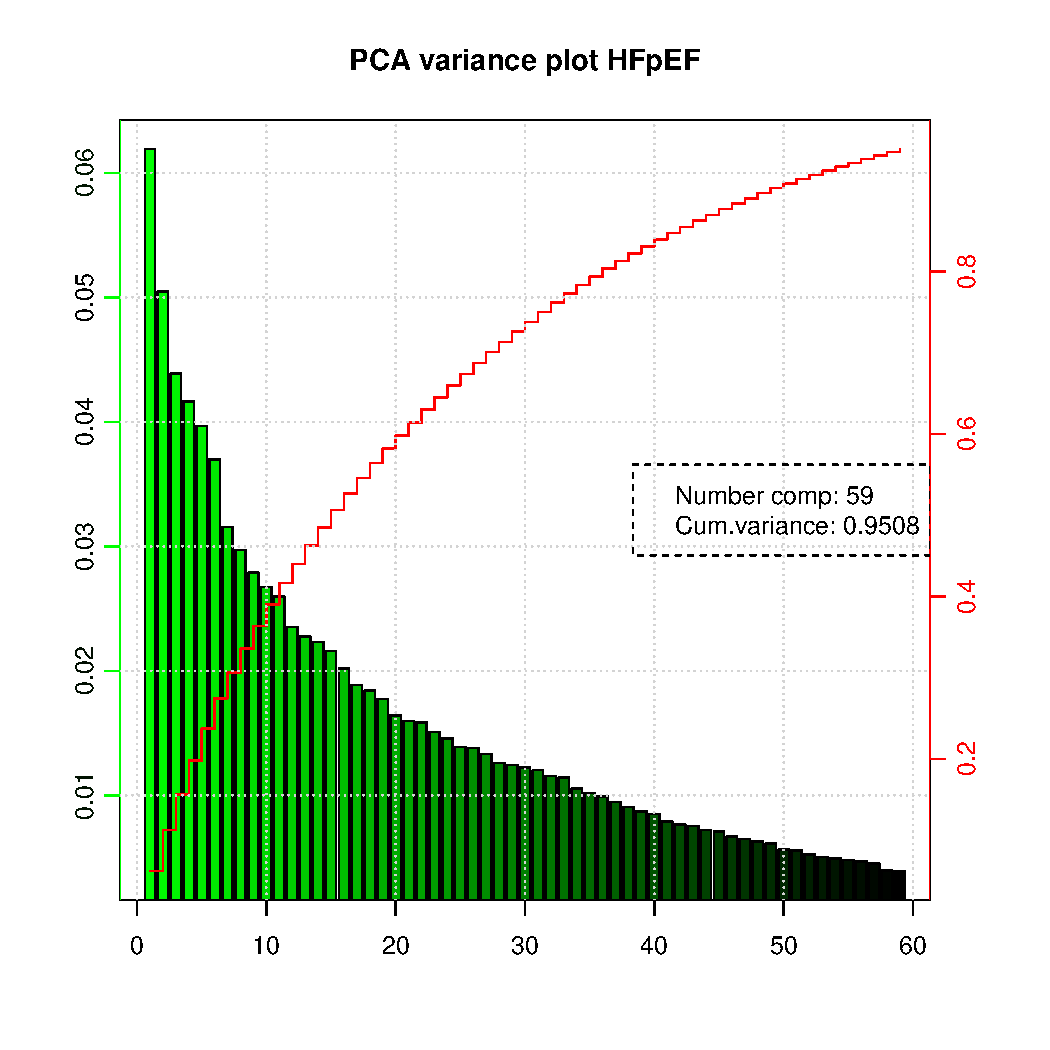
\includegraphics[width=1.15\textwidth]{doc/thesis/images/pca_var_plot_HFpEF.pdf}
\end{figure}


\chapter{Source Code}
\label{chap:souce_code}

\noindent The following appendix presents all the relevant \texttt{R}-code used in this thesis. We have organized the chapter in accordance with the various steps in the machine learning procedure adopted in this thesis, see figure (\ref{fig:ML_proc_thesis}). We have tried to comment as much of the source code in order to ensure that an eventual re-examination of the results can be as easy and smooth as possible. Inquires about the code can be forwarded to the author on request.

\section{Helper Functions, \texttt{\_helper\_func.R}}
\label{sec:helper_func}

\lstinputlisting[language=R]{../../data/data_sets/source/_helper_func.R}

\section{Load Data and Labeling, \texttt{r\_data\_sets.R}}
\label{sec:load_data}

\lstinputlisting[language=R]{../../data/data_sets/raw_data/r_data_sets.R}

\section{Data Description, \texttt{desc\_data.R}}
\label{sec:app_desc_stat}

\lstinputlisting[language=R]{../../data/data_sets/source/desc_data.R}

\section{Imputation, \texttt{imputation.R}}
\label{sec:app_impu}

\lstinputlisting[language=R]{../../data/data_sets/source/imputation.R}

\section{Dimensional Reduction, \texttt{dim\_reduc.R}}
\label{sec:dim_red}


\end{document}